\section{Forschungsmethode}
Den Richtlinien in \cite{Keele2007GuidelinesEngineering} folgend, wurde ein Systematisches Literatur Review (SLR) nach Kitchenham et al. durchgeführt. Das Dokument folgt dem Aufbau in \cite{Walia2009AErrors}. Dieser SLR umfasst die folgenden Schritte

\begin{itemize}
    \item Formulierung eines Review-Protokolls
    \item Durchführen des Reviews
        \begin{itemize}
            \item Identifizierung von Primärstudien
            \item Evaluierung \& Auswahl
            \item Datenextraktion
            \item Datensynthese
        \end{itemize}
    \item Analyse der Ergebnisse
    \item Auswertung der Ergebnisse
\end{itemize}

Ein Review Protokoll enthält Forschungsfragen, Methoden, Vorgehensweisen etc. die benötigt werden, um ein SLR durchführen zu können. Es ist notwendig um zu vermeiden, das die Forschung durch die Erwartungshaltung des Forschers getrieben wird und an Objektivität verliert (Researcher bias). Nach der Durchführung erfolgt die Analyse und Auswertung der Ergebnisse um die Forschungsfragen und die übergeordnete Forschungsfrage zu beantworten.

\subsection{Forschungsfragen}

Das Hauptaugenmerk dieses SLR war es, bestehende Probleme in der Requirements Traceability zu identifizieren und zu klassifizieren. Um einen Fokus zu setzen, wurde sich bei den Forschungfragen am untergeordneten Ziel, der Verbesserung der Erkennung und Vermeidung von Qualitätsproblemen in der Requirements Traceability, orientiert. Das Hauptziel dieses Reviews war:

\begin{center}
\enquote{Welche Arten von Problemen existieren im Management von Requirements Traceability und wie können diese klassifiziert werden?}
\end{center}


\\
\\
DRAFT für die Bestimmung von Forschungsfragen nach dem das Review durchgeführt werden soll
Klassifikation

\begin{figure}[!htb]
  \centering
  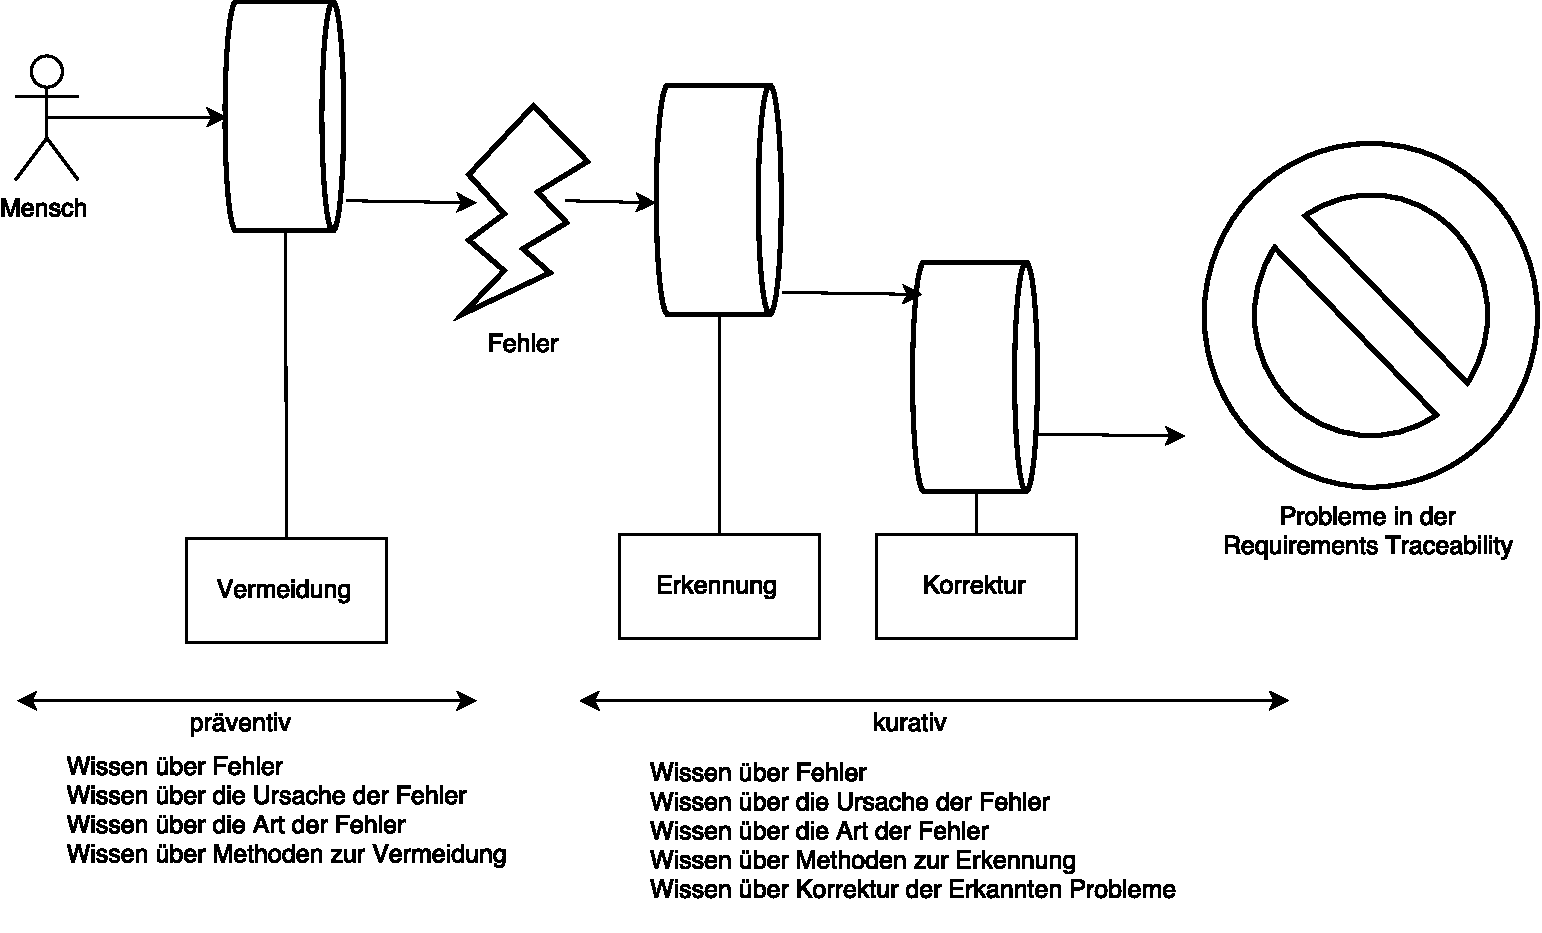
\includegraphics[width=3.4in]{Draft_Klassifikation_SLR.pdf}
  \caption{Draft Klassifikation für Forschungsfragen}
  \label{fig:abb3}
\end{figure}


